\section{Erweiterung des Definitionsbereich der Exponentialfunktion}
Mit der Darstellung der Exponentialfunktion $\R \to \R,\, x\mapsto e^x$ als unendliche Reihe $e^x = 1 + \frac{x}{1!}+ \frac{x^2}{2!}+ \frac{x^3}{3!}+\cdots$ lässt sich die Funktion auf andere Mengen ausweiten. Zum Beispiel auf die komplexen Zahlen.

\begin{LA}{Repetition der komplexen Zahlen}{}
	In der zweiten Klasse haben Sie die komplexen Zahlen bereits kennengelernt. Mit diesen Aufgaben soll ein Teil dieses Wissens wieder in Erinnerung gerufen werden.



	\begin{enumerate}
		\item $z = 12 - 5i, \quad \operatorname{Re}(z) =?, \quad \operatorname{Im}(z) = ? , \quad |z| = ?, \quad \bar{z}=?$

		\item $z = 3 + 4i, \quad i\cdot z = ?$

		\item \((8+2i)(7+3i)\)


		      %\item \(\frac{5+2i}{-3+5i}\)


		\item \(i^2=?,\quad i^3=?,\quad i^4=?,\quad i^5 =?,\quad i^{243} = ? \)

		\item Wie lautet die Normalform der Zahl $z = 2\cis\left(\frac{\pi}{4}\right)$?

		\item Geben Sie die Polarform von \(-2+2\sqrt{3}i\) an.

		\item Berechnen Sie: $3\operatorname{cis}\left(\frac{\pi}{4}\right) \cdot 4\operatorname{cis}\left(\frac{7\pi}{12}\right)$





		      % \item \(z = 4 \operatorname{cis} \left(\frac{\pi}{3}\right)\). Bestimmen Sie die Polarform von \(-z\) und \(\bar{z}\).


		      %\item Lösen Sie die Gleichung \(z^2 = i\). Verwenden Sie für solche Fragen die Polarform.


		      %\item Lösen Sie die Gleichung \(z^5 = 1\). Stellen Sie die Lösungen als Punkte in der Zahlenebene dar.


		      %\item \(z_0 = \sqrt{3} - i\) ist eine Lösung von \(z^4 = a\). Berechnen Sie \(a\) und die übrigen Lösungen.



		      % \item Finden Sie alle Lösungen der Gleichung \(z^4 - z^3 - 3z + 3 = 0\). Tipp: Zeigen Sie zuerst, dass \(z = 1\) eine Lösung ist und führen Sie anschliessend eine Polynomdivision durch.

	\end{enumerate}
\end{LA}

% \clearpage
% \emph{Lösungen}


%     \begin{enumerate}
%         \item $z = 12 - 5i, \quad \operatorname{Re}(z) =12, \quad \operatorname{Im}(z) = -5 , \quad |z| = 13, \quad \bar{z}=12+5i$
%      \item $iz =  -4+3i$
%     \item $50+38i$
%     %\item $-\frac{5}{34} - \frac{31}{34}i$
%     \item \(i^2=-1,\quad i^3=-i,\quad i^4=1,\quad i^5 =i,\quad i^{243} = -i \)
%     \item $z = 2\cis\left(\frac{\pi}{4}\right) = \sqrt{2} + \sqrt{2}i$


%     \item $4 \operatorname{cis}\left(\frac{2\pi}{3}\right)$
%      \item $12\operatorname{cis}\left(\frac{5\pi}{6}\right) =-6\sqrt{3}+6 i $
%     %\item  $-z = 4 \operatorname{cis}\left(\frac{4\pi}{3}\right), \quad \bar{z} = 4 \operatorname{cis}\left(\frac{5\pi}{3}\right)$

%     %\item $\operatorname{cis}\left(\frac{\pi}{4}\right)$ und $\operatorname{cis}\left(\frac{5\pi}{4}\right)$
%    % \item $1, \operatorname{cis}\left(\frac{2\pi}{5}\right), \operatorname{cis}\left(\frac{4\pi}{5}\right), \operatorname{cis}\left(\frac{6\pi}{5}\right), \operatorname{cis}\left(\frac{8\pi}{5}\right)$
%     %\item $a = -8 - 8\sqrt{3}i$, weitere Lösungen: $z_1 = -z_0$ und $z_2, z_3 = \pm (2 \operatorname{cis}\left(\frac{7\pi}{3}\right))$

%     %\item $z_1 = 1$, $z_2 = \sqrt[3]{3}$, $z_3 = \sqrt[3]{3} \operatorname{cis}\left(\frac{2\pi}{3}\right)$, $z_4 = \sqrt[3]{3} \operatorname{cis}\left(\frac{4\pi}{3}\right)$
% \end{enumerate}



% \subsection{Repetition: komplexe Zahlen}

% In der zweiten Klasse haben Sie die komplexen Zahlen bereits kennengelernt. In diesem Abschnitt soll dieses Wissen wieder in Erinnerung gerufen werden.

% Dazu können Sie direkt die folgenden Übungen probieren. 

% \begin{LA}
%     {Repetitionsaufgaben zu komplexen Zahlen}{}



%     \begin{enumerate}
%         \item Berechnen Sie:
%         \begin{enumerate}
%             \item $z = 3 + 4i, \quad \bar{z} = ?$

%         \item \((8+2i)(7+3i)\)


%         \item \(\frac{5+2i}{-3+5i}\)


%         \item \(i^{243}\)

%         \item $3\operatorname{cis}\left(\frac{\pi}{4}\right) \cdot 4\operatorname{cis}\left(\frac{7\pi}{12}\right)$
%     \end{enumerate}


%         \item Geben Sie die Polarform von \(-2+2\sqrt{3}i\) an.

%         \item \(z = 4 \operatorname{cis} \left(\frac{\pi}{3}\right)\). Bestimmen Sie die Polarform von \(-z\) und \(\bar{z}\).


%         \item Lösen Sie die Gleichung \(z^2 = i\). Verwenden Sie für solche Fragen die Polarform.


%         %\item Lösen Sie die Gleichung \(z^5 = 1\). Stellen Sie die Lösungen als Punkte in der Zahlenebene dar.


%         \item \(z_0 = \sqrt{3} - i\) ist eine Lösung von \(z^4 = a\). Berechnen Sie \(a\) und die übrigen Lösungen.



%        % \item Finden Sie alle Lösungen der Gleichung \(z^4 - z^3 - 3z + 3 = 0\). Tipp: Zeigen Sie zuerst, dass \(z = 1\) eine Lösung ist und führen Sie anschliessend eine Polynomdivision durch.

%     \end{enumerate}
% \end{LA}
% \clearpage
% \emph{Lösungen}

% \begin{enumerate}
%     \item Berechnungen
%     \begin{enumerate}
%      \item   $\bar{z} =  3-4i$
%     \item $50+38i$
%     \item $-\frac{5}{34} - \frac{31}{34}i$
%     \item $-i$
%     \item $12\operatorname{cis}\left(\frac{5\pi}{6}\right) =-6\sqrt{3}+6 i $
%     \end{enumerate}
%     \item $4 \operatorname{cis}\left(\frac{2\pi}{3}\right)$
%     \item  $-z = 4 \operatorname{cis}\left(\frac{4\pi}{3}\right), \quad \bar{z} = 4 \operatorname{cis}\left(\frac{5\pi}{3}\right)$

%     \item $\operatorname{cis}\left(\frac{\pi}{4}\right)$ und $\operatorname{cis}\left(\frac{5\pi}{4}\right)$
%    % \item $1, \operatorname{cis}\left(\frac{2\pi}{5}\right), \operatorname{cis}\left(\frac{4\pi}{5}\right), \operatorname{cis}\left(\frac{6\pi}{5}\right), \operatorname{cis}\left(\frac{8\pi}{5}\right)$
%     \item $a = -8 - 8\sqrt{3}i$, weitere Lösungen: $z_1 = -z_0$ und $z_2, z_3 = \pm (2 \operatorname{cis}\left(\frac{7\pi}{3}\right))$

%     %\item $z_1 = 1$, $z_2 = \sqrt[3]{3}$, $z_3 = \sqrt[3]{3} \operatorname{cis}\left(\frac{2\pi}{3}\right)$, $z_4 = \sqrt[3]{3} \operatorname{cis}\left(\frac{4\pi}{3}\right)$
% \end{enumerate}


% \clearpage

% In den folgenden Teilkapitel werden die wichtigsten Definitionen und Sätze über komplexe Zahlen in kürze repetiert. Sie können diese Abschnitte überspringen und nur nach Bedarf etwas nachschlagen. 
% \subsubsection{Grundsätzliches}


% \begin{definition}
%     {Komplexe Zahl}{}
%     Die imaginäre Einheit \(i\) ist eine Zahl mit der Eigenschaft, dass \(i^2 = -1\). Eine komplexe Zahl ist eine Zahl der Form \(z = a + b \cdot i\), wobei \(a, b \in \mathbb{R}\). Die Menge der komplexen Zahlen wird mit \(\mathbb{C}\) bezeichnet. Die reellen Zahlen \(a\) und \(b\) nennt man den Realteil respektive den Imaginärteil von \(z\). Die Notation dafür lautet: \(a = \operatorname{Re}(z)\), \(b = \operatorname{Im}(z)\).

% \end{definition}

% Die Addition und Multiplikation komplexer Zahlen werden so definiert, dass die Rechengesetze Assoziativität, Kommutativität und Distributivität weiterhin gelten:
% \begin{definition}
%     {Addition und Multiplikation}{}
%     Für zwei komplexe Zahlen der Form \(z = a + b \cdot i\) und \(w = x + y \cdot i\) sei
% \[z + w = (a + x) + (b + y) \cdot i\]
% \[z \cdot w = (ax - by) + (ay + bx) \cdot i\]

% \end{definition}
% Zwei wichtige Begriffe rund um komplexe Zahlen sind der Betrag und konjugiert komplexe Zahlen:
% \begin{definition}
%     {Betrag und konjugierte Zahl}{}
%     Sei \(z = a + b \cdot i\).
% Die zu \(z\) konjugiert komplexe Zahl ist \(\bar{z} = a - b \cdot i\).
% Der Betrag von \(z\) ist definiert als: \(|z| = \sqrt{z \cdot \bar{z}} = \sqrt{a^2 + b^2} \in \mathbb{R}\).

% \end{definition}
% Mithilfe der konjugiert komplexen Zahlen lassen sich Divisionen in $\C$ durchführen.

% \begin{bsp}
%     {Division komplexer Zahlen}{}
%     \[\frac{1 + 3i}{3 + 4i} = \frac{(1 + 3i)(3 - 4i)}{(3 + 4i)(3 - 4i)} = \frac{3 - 4i + 9i - 12i^2}{9 - 16i^2} = \frac{15 + 5i}{25} = \frac{3}{5} + \frac{1}{5}i\]

% \end{bsp}
% \begin{satz}
%     {Fundamentalsatz der Algebra}{}
%     Ein Polynom lässt sich in $\C$ vollständig in Linearfaktoren zerlegen.

%     Daraus folgt, dass eine Gleichung $n$-ten Grades immer genau $n$ Nullstellen hat (unter Berücksichtigung der Vielfachheit).
% \end{satz}
% \begin{bsp}
%     {Zerlegung eines Polynoms}{}
%     \[x^3 - x^2 + x - 1 = (x - 1)(x^2 + 1) = (x - 1)(x + i)(x - i)\]
%     Die Gleichung 3. Grades $x^3 - x^2 + x - 1 = 0$ hat dann die Nullstellen $x_1=1, x_2=-i, x_3=i$
% \end{bsp}

% \begin{satz}
%     {Nullstellen reeller Polynome}{}
%     Ist $z$ die Nullstelle eines Polynoms mit reellen Koeffizienten, so ist auch $\bar z$ eine Nullstelle.
% \end{satz}
% \begin{bsp}
%     {}{}
%     $x^2 + 4x + 8$ hat die Nullstellen $ -2 + 2i$  und  $-2 - 2i$.
% \end{bsp}

% \subsubsection{Die Gauss'sche Zahlenebene}
% \begin{definition}
%     {Die Zahlenebene}{}
%     Die Menge der komplexen Zahlen kann als eine Ebene dargestellt werden. Dabei wird die komplexe Zahl \(z = a + b \cdot i\) durch den Punkt \(P(a \vert b)\) dargestellt. Diese Darstellung von \(\mathbb{C}\) nennt man die Gausssche Zahlenebene. Die horizontale Achse nennt man reelle Achse, die vertikale imaginäre Achse.
%     % \begin{center}
%     %     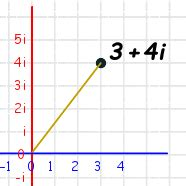
\includegraphics[scale = 0.5]{media/bspkomplexezahl.jpeg}
%     % \end{center}$
%     \begin{center}
%         \begin{tikzpicture}[scale=0.4]
%             % Gitter
%             \draw[dashed, very thin, gray] (-5,-5) grid (5,5);

%             % Achsen mit Skala
%             \draw[->] (-5,0) -- (5,0) node[right] {Reelle Achse};
%             \draw[->] (0,-5) -- (0,5) node[right] {Imaginäre Achse};
%             \foreach \x in {-4,-3,-2,-1,1,2,3,4} 
%                 \draw (\x,0) -- (\x,-0.2) node[below] {$\x$};
%              \foreach \y in {-4,-3,-2,2,3,4}
%                 \draw (0,\y) -- (-0.2,\y) node[left] {$\y i$};
%             \draw (0,1) -- (-0.2,1) node[left] {$i$};
%             %\draw (0,-1) -- (-0.2,-1) node[left] {$-i$};

%             % Punkte und Markierungen
%             %\draw[dashed, very thin, gray] (2,0) -- (2,3) -- (0,3);
%             \fill[red] (0,1) circle (0.1) node[right] {$z = i$};
%             \fill[purple] (2,3) circle (0.1) node[right] {$w = 2 + 3i$};
%         \end{tikzpicture}
%     \end{center}


% \end{definition}

% Die Gauss'sche Zahlenebene ermöglicht eine geometrische Deutung der Operationen mit komplexen Zahlen:

% \begin{satz}
%     {Geometrische Sicht auf die Addition von komplexen Zahlen}{}
%     Die Addition zweier komplexen Zahlen \(z = a + b \cdot i\) und \(w = x + y \cdot i\) entspricht der Addition der Ortsvektoren \(\vec{z} = \begin{pmatrix} a \\ b \end{pmatrix}\) und \(\vec{w} = \begin{pmatrix} x \\ y \end{pmatrix}\). Das Gleiche gilt für die Subtraktion.
%     % \begin{center}
%     %     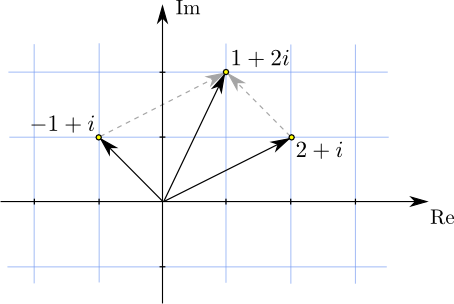
\includegraphics[width = 0.5 \textwidth]{media/additioninC.png}
%     % \end{center}
%     \begin{center}

%         Addition

%         \begin{tikzpicture}[scale = 1]


%             % Achsen mit Skala
%             \draw[->, thick] (-1.5,0) -- (4.5,0) node[above] {$\RE$};
%             \draw[->, thick] (0,-1.5) -- (0,2.5) node[right] {$\IM$};
%             \foreach \x in {-1,2,3,4} 
%                 \draw (\x,0.1) -- (\x,-0.1) ;
%             \foreach \y in {-1,2,} 
%                 \draw (0.1,\y) -- (-0.1,\y) ;
%             \draw (0.1,1) -- (-0.1,1) node[left] {$i$};
%             \draw (1,0.1) -- (1,-0.1) node[below] {$1$};

%              % Vektoren
%              \draw[->, thick, dashed] (0,0) -- node[above] {$\vec{z}_1$} ++(1,5/4) node[above left, ForestGreen] {$z_1 = a + bi$};
%              \draw[->, thick, dashed] (0,0) -- node[below right] {$\vec{z}_2$} ++(2,3/4) node[below right, ForestGreen] {$z_2 = c + di$};
%              \draw[->, thick, orange] (0,0) -- (3,2) node[above right, orange] {$z_1 + z_2$};
%              \draw[->, thick, dashed] (1,5/4) -- (3,2) ; 
%              \draw[->, thick, dashed] (2,3/4) -- (3,2) ; 

%              % Punkte
%              \fill[ForestGreen] (1,5/4) circle (0.05);
%              \fill[ForestGreen] (2,3/4) circle (0.05) ;
%              \fill[orange] (3,2) circle (0.05);
%         \end{tikzpicture}

%     \end{center}

% \end{satz}
% Zur geometrischen Deutung der Multiplikation benötigen wir eine andere Darstellung der komplexen Zahlen.
% \subsubsection{Die Polarform einer komplexen Zahl}
% Mit Ausnahme von 0 kann jeder Punkt der (Zahlen)Ebene eindeutig durch seinen Abstand zum Ursprung und dem Winkel zwischen dem entsprechenden Ortsvektor und der reellen Achse angegeben werden.
% \begin{definition}
%     {Polarform}{}
%     Die Polarform einer komplexen Zahl \(z = x + yi\) lautet \(z = r \operatorname{cis} \varphi\). Dabei ist \(r > 0\) der Abstand vom Ursprung und \(\varphi\) der Winkel zwischen dem Ortsvektor und der positiven x-Achse. Die Form \(z = x + yi\) nennt man die kartesische Form.
%     % \begin{center}
%     %     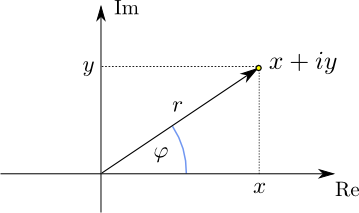
\includegraphics[scale = 0.5]{media/polarform.png}
%     % \end{center}
%     \begin{center}
%         \begin{tikzpicture}[scale = 0.7]
%             % Achsen mit Skala
%             \draw[->, thick] (-1.5,0) -- (4.5,0) node[above] {$\operatorname{Re}$};
%             \draw[->, thick] (0,-1.5) -- (0,2.5) node[right] {$\operatorname{Im}$};
%             \foreach \x in {-1,2,3,4} 
%                 \draw (\x,0.1) -- (\x,-0.1) ;
%             \foreach \y in {-1,2,} 
%                 \draw (0.1,\y) -- (-0.1,\y) ;
%             \draw (0.1,1) -- (-0.1,1) node[left] {$i$};
%             \draw (1,0.1) -- (1,-0.1) node[below] {$1$};

%             % Vektoren
%             \draw[->, thick] (0,0) -- node[above] {$r$}  ++(2.5, 2) ;

%             % Punkte
%             \fill[ForestGreen] (2.5,2) circle (0.05) node[above, ForestGreen] {$z$};

%             % Winkel
%             \draw[thick, ->] (1.2,0) arc (0:38:1.2) node[midway, right] {$\varphi$};

%         \end{tikzpicture}   
%     \end{center}

% \end{definition}
% Der folgende Satz erklärt, wie man die Polarform aus der kartesischen Form ermittelt und umgekehrt.


% \begin{satz}
%     {Umwandlung kartesische Form und Polarform}{}
%     Es gelten folgende Umrechnungsformeln für \(z = x + yi = r \operatorname{cis} (\varphi)\):


% \begin{align*}
% x &= r \cos \varphi \\
% y &= r \sin \varphi
% \end{align*}


% und

% \begin{align*}
% r &= |z| = \sqrt{x^2 + y^2} \\
% \varphi &= 
% \begin{cases}
% \arctan \left(\frac{y}{x}\right), & \text{falls } x > 0 \\
% \pi + \arctan \left(\frac{y}{x}\right), & \text{falls } x < 0
% \end{cases}
% \end{align*}


% \end{satz}

% \emph{Bemerkung:} $\operatorname{cis} (\varphi)$ ist eine Abkürzung für $\cos \varphi + i \sin \varphi$

% Komplexe Zahlen in Polarform lassen sich einfach multiplizieren:
% \begin{satz}
%     {Multiplikation in Polarform}{}
%     Sei \(z = r_1 \operatorname{cis} \varphi_1\), \(w = r_2 \operatorname{cis} \varphi_2\).
% Dann gilt:
% \[z \cdot w = r_1 r_2 \operatorname{cis} (\varphi_1 + \varphi_2)\]

% \[\frac{z}{w} = \frac{r_1}{r_2} \operatorname{cis} (\varphi_1 - \varphi_2)\]

% \[z^n = r_1^n \operatorname{cis}(n \varphi_1)\]
% % \begin{center}
% %     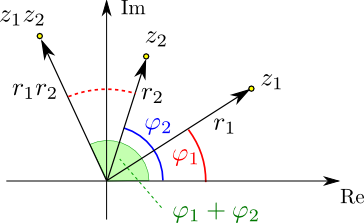
\includegraphics[scale = 0.5]{media/multiplikation-461714259.png}
% % \end{center}

% \begin{center}
%     \begin{tikzpicture}[scale = 1]
%         % Gitter
%         \draw[dashed, very thin, gray] (-4,-4) grid (4,4);

%         % Achsen mit Skala
%         \draw[->] (-4,0) -- (4,0) node[above] {$\RE$};
%         \draw[->] (0,-4) -- (0,4) node[right] {$\IM$};
%         \foreach \x in {-3,-2,-1,1,2,3} 
%             \draw (\x,0) -- (\x,-0.2) ;
%          \foreach \y in {-3,-2, -1,2,3}
%             \draw (0,\y) -- (-0.2,\y) ;
%         \draw (0,1) -- (-0.2,1) node[left] {$i$};
%         \draw (1,0) -- (1,-0.2) node[below] {$1$};


%         % Punkt z1
%         \coordinate (z1) at (60:1.5);
%         \fill[ForestGreen] (z1) circle (0.05) node[above, ForestGreen] {$z_1$};
%         \draw[ForestGreen](0,0) -- (z1);
%         \draw[thick, ->, ForestGreen] (1, 0) arc (0:60:1) node[midway, left] {$\varphi_1$};

%          % Punkt z
%          \coordinate (z) at (130:2);
%          \fill[blue] (z) circle (0.05) node[above, blue] {$z$};
%          \draw[blue](0,0) -- (z);
%          \draw[thick, ->, blue] (1.2, 0) arc (0:130:1.2) node[midway, above left] {$\varphi$};
%          \draw[dashed] (0,0) circle (2);

%          % Punkt z_1*z
%          \coordinate (z1z) at (190:3);
%          \fill[red] (z1z) circle (0.05) node[below, red] {$z_1\cdot z$};
%          \draw[red](0,0) -- (z1z);
%          \draw[thick, ->, red] (130:1.2) arc (130:190:1.2) node[midway, left] {$\varphi_1$};


%     \end{tikzpicture}   
% \end{center}


% \end{satz}
% \begin{bsp}
%     {Rein kubische Gleichung}{}
%     Die Gleichung \(z^3 = -27\) hat in \(\mathbb{C}\) drei Lösungen. Diese findet man am einfachsten, indem man die Polarform verwendet. Sei \(z = r \operatorname{cis}(\varphi)\). Dann ist \(z^3 = r^3 \operatorname{cis}(3\varphi)\). Weiter ist \(-27 = 27 \operatorname{cis}(\pi)\). Also gilt
% \[r^3 \operatorname{cis}(3\varphi) = 27 \operatorname{cis}(\pi)\]

% Daraus folgt
% \[
% \begin{cases}
%     r^3 = 27 \\
%     3\varphi \equiv \pi \pmod{2\pi}
% \end{cases}
% \]

% Daraus ergibt sich
% \[r = 3 \quad \text{und} \quad \varphi = \frac{\pi}{3} \text{ oder } \pi \text{ oder } \frac{5\pi}{3}\]

% Die Lösungen lauten also
% \[z_1 = 3 \operatorname{cis}\left(\frac{\pi}{3}\right), \quad z_2 = 3 \operatorname{cis}(\pi) = -3, \quad z_3 = 3 \operatorname{cis}\left(\frac{5\pi}{3}\right)\]


% \end{bsp}



% \clearpage
%\subsection{Die Exponentialfunktion auf \texorpdfstring{$\C$}{C}}


\clearpage
Mit komplexen Zahlen kann man die vier Grundoperationen ausführen und in den vergangenen Kapitel haben wir gelernt, wie man einige Funktionen wie Sinus, Cosinus und die Funktion $f(x)=e^x$ genau mit diesen vier Grundoperationen berechnen kann. Damit lassen sich diese Funktionen so erweitern, dass auch komplexe Zahlen als Inputs möglich sind!

\begin{definition}
	{}{Die Exponentialfunktion für komplexe Argumente}
	Für \(z \in \mathbb{C}\) sei
	\[e^z = \sum_{k=0}^{\infty} \frac{z^k}{k!} = 1 + \frac{z}{1!} + \frac{z^2}{2!} + \ldots\]

\end{definition}

\begin{bsp}
	{$e^i$}{}
	\[e^i = 1 + \frac{i}{1!} + \frac{i^2}{2!} + \frac{i^3}{3!} + \frac{i^4}{4!} + \frac{i^5}{5!} + \ldots
		%= 1 + i - \frac{1}{2} - \frac{i}{6} + \frac{1}{24} + \frac{i}{120} - \ldots 
		\approx 0.54 + 0.84i\]

\end{bsp}
Der Schweizer Mathematiker Leonhard Euler (1707-1783) gehört zu den bedeutendsten Persönlichkeiten in der Geschichte der Mathematik. In seinem Werk \textit{Introductio in analysin infinitorum}, das 1748 erschienen ist, beweist er die sogenannte Eulersche Formel, die einen Zusammenhang zwischen der komplexen Exponentialfunktion und den trigonometrischen Funktionen herstellt. Eine Folgerung davon ist die berühmte Eulersche Identität, welche eine wahrhaft erstaunliche Beziehung zwischen den fünf wichtigsten Zahlen aufdeckt.


\begin{figure}[h]
	\begin{center}
		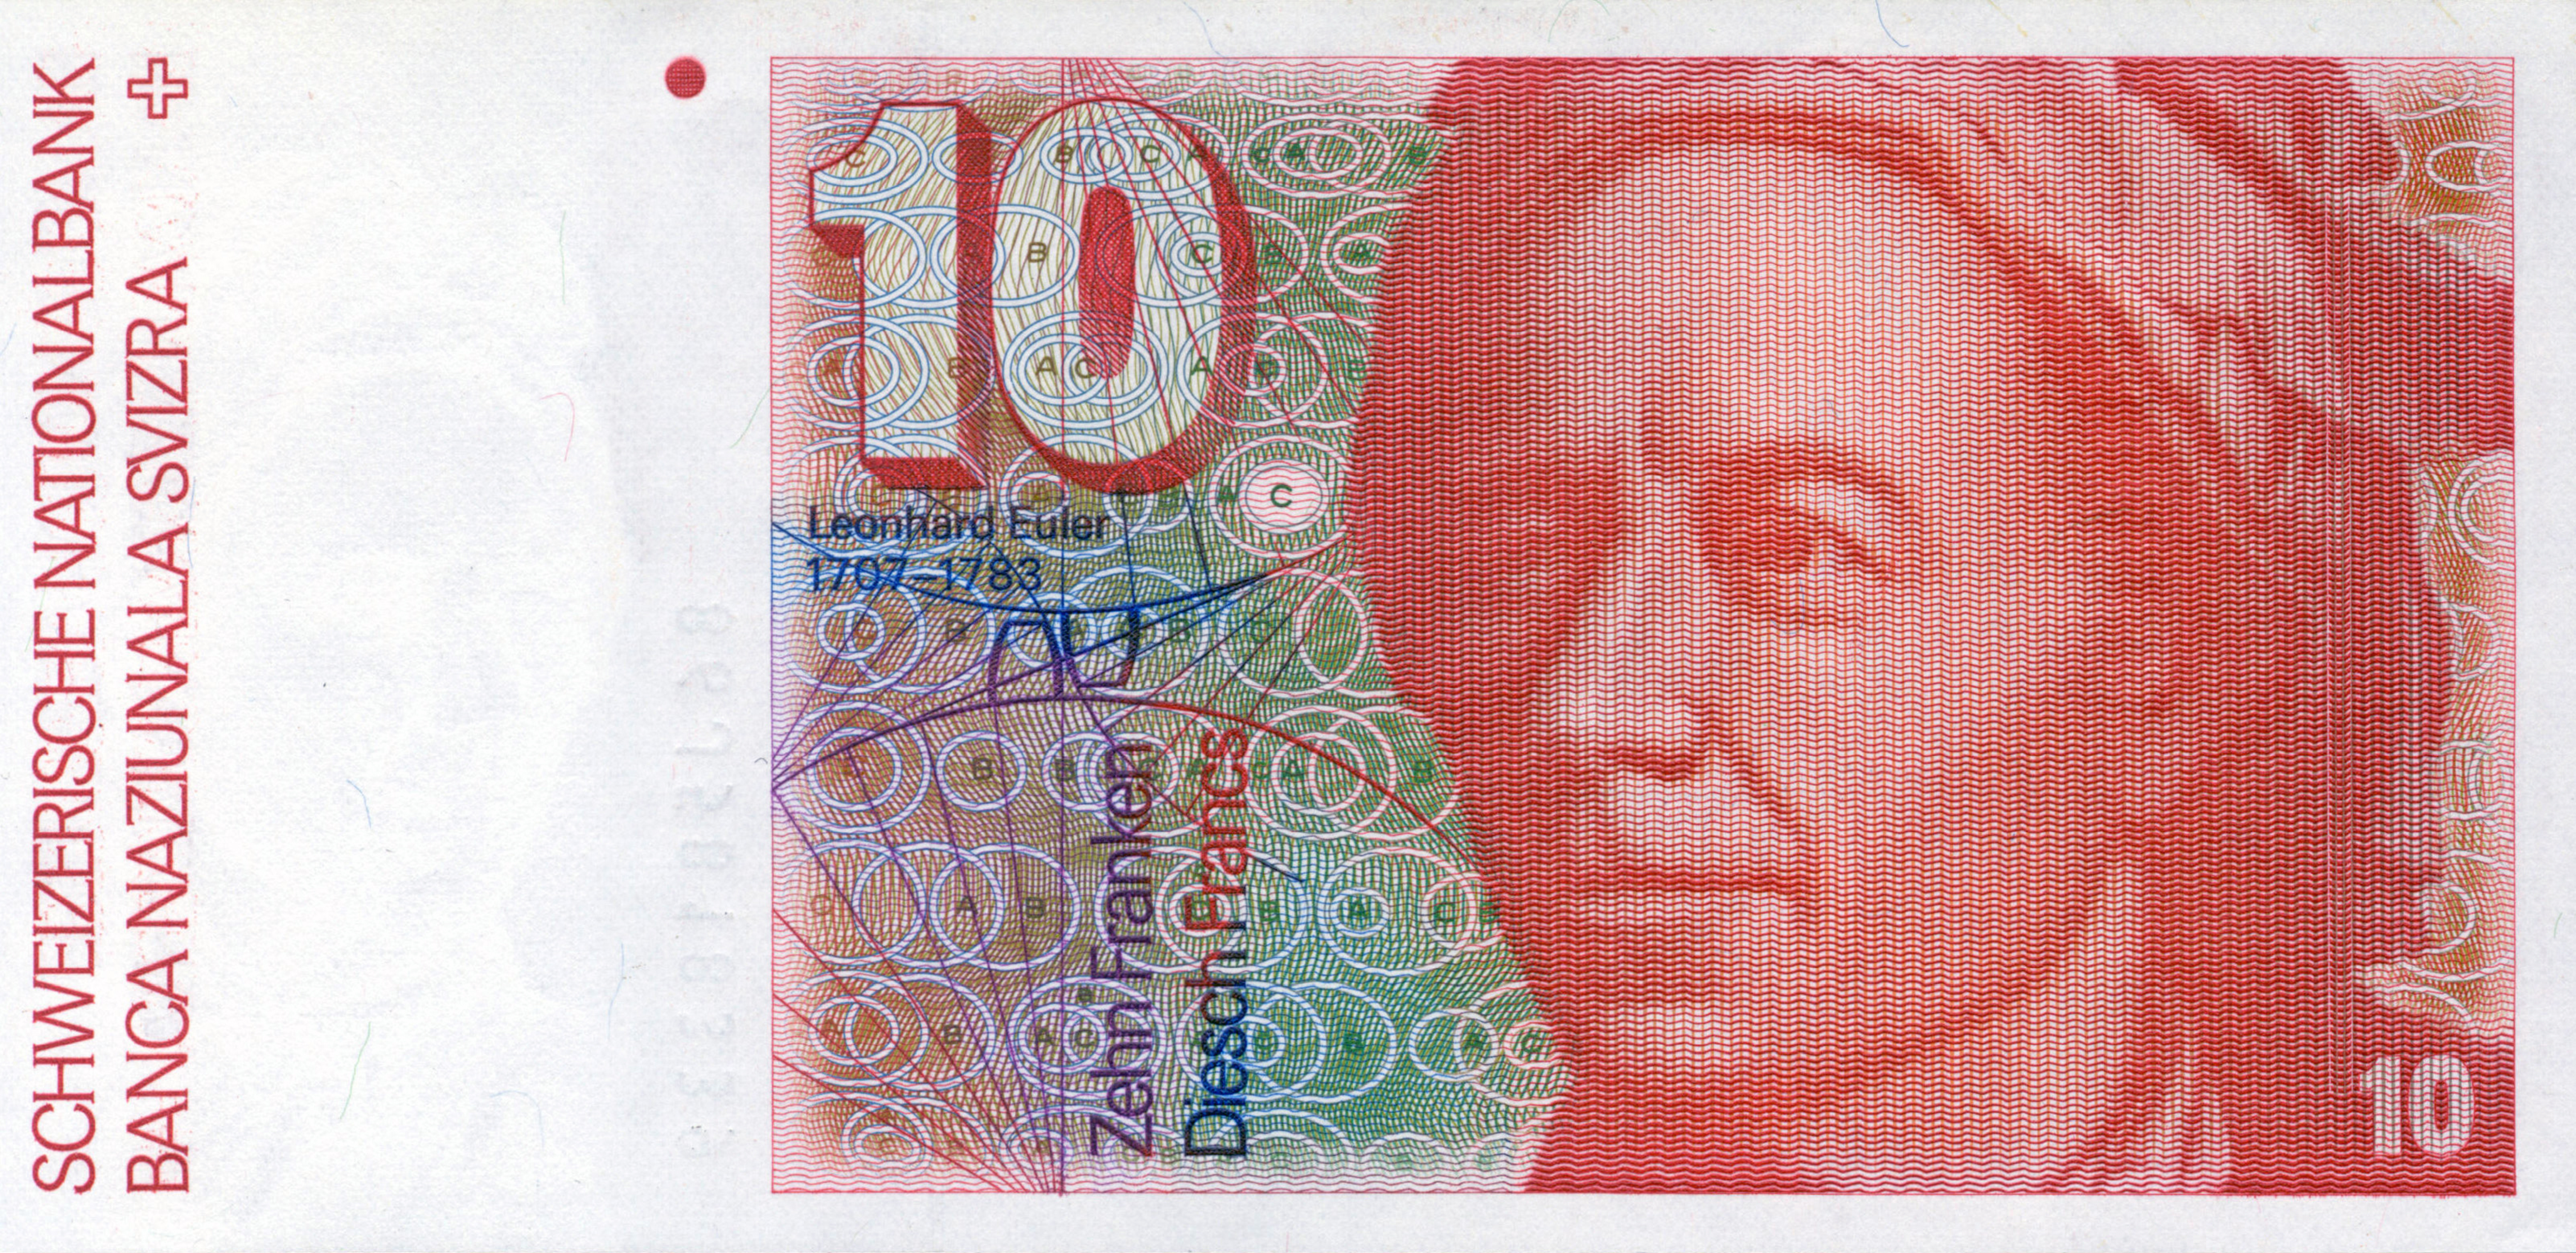
\includegraphics[width = 0.6 \textwidth]{media/Euler-10_Swiss_Franc_banknote_(front).pdf}
		\caption{Schweizer 10-Franken-Note bis 1995}
	\end{center}
\end{figure}



\begin{LA}
	{Entdecken Sie die Eulersche Formel und die Eulersche Identität}{}
	\begin{enumerate}
		\item Berechnen Sie eine Näherung für \(e^{i \pi / 2}\), indem Sie die ersten 6 Summanden der Summe in der Definition berechnen. (Kontrolle: \(e^{i \pi / 2}\approx 0.0200 + 1.0045 i \))
		\item  Sei \(x \in \mathbb{R}\). Stellen Sie die Summe für die Zahl \(e^{i \cdot x}\) auf und vereinfachen Sie den Real- und Imaginärteil. Am Schluss sollten Sie ein schönes Resultat erhalten: Die Eulersche Formel!
		\item   Bestimmen Sie mit der Formel aus 2. die Zahl \(e^{i \pi}\).
	\end{enumerate}



\end{LA}

\clearpage
\begin{satz}
	{Eulersche Identität und Eulersche Formel}{}
	Sei \(\varphi \in \mathbb{R}\). Dann gilt
	\[e^{i \cdot \varphi} =\phantom{\cos(\varphi) + i \cdot \sin (\varphi)}\]
	% \begin{center}
	%     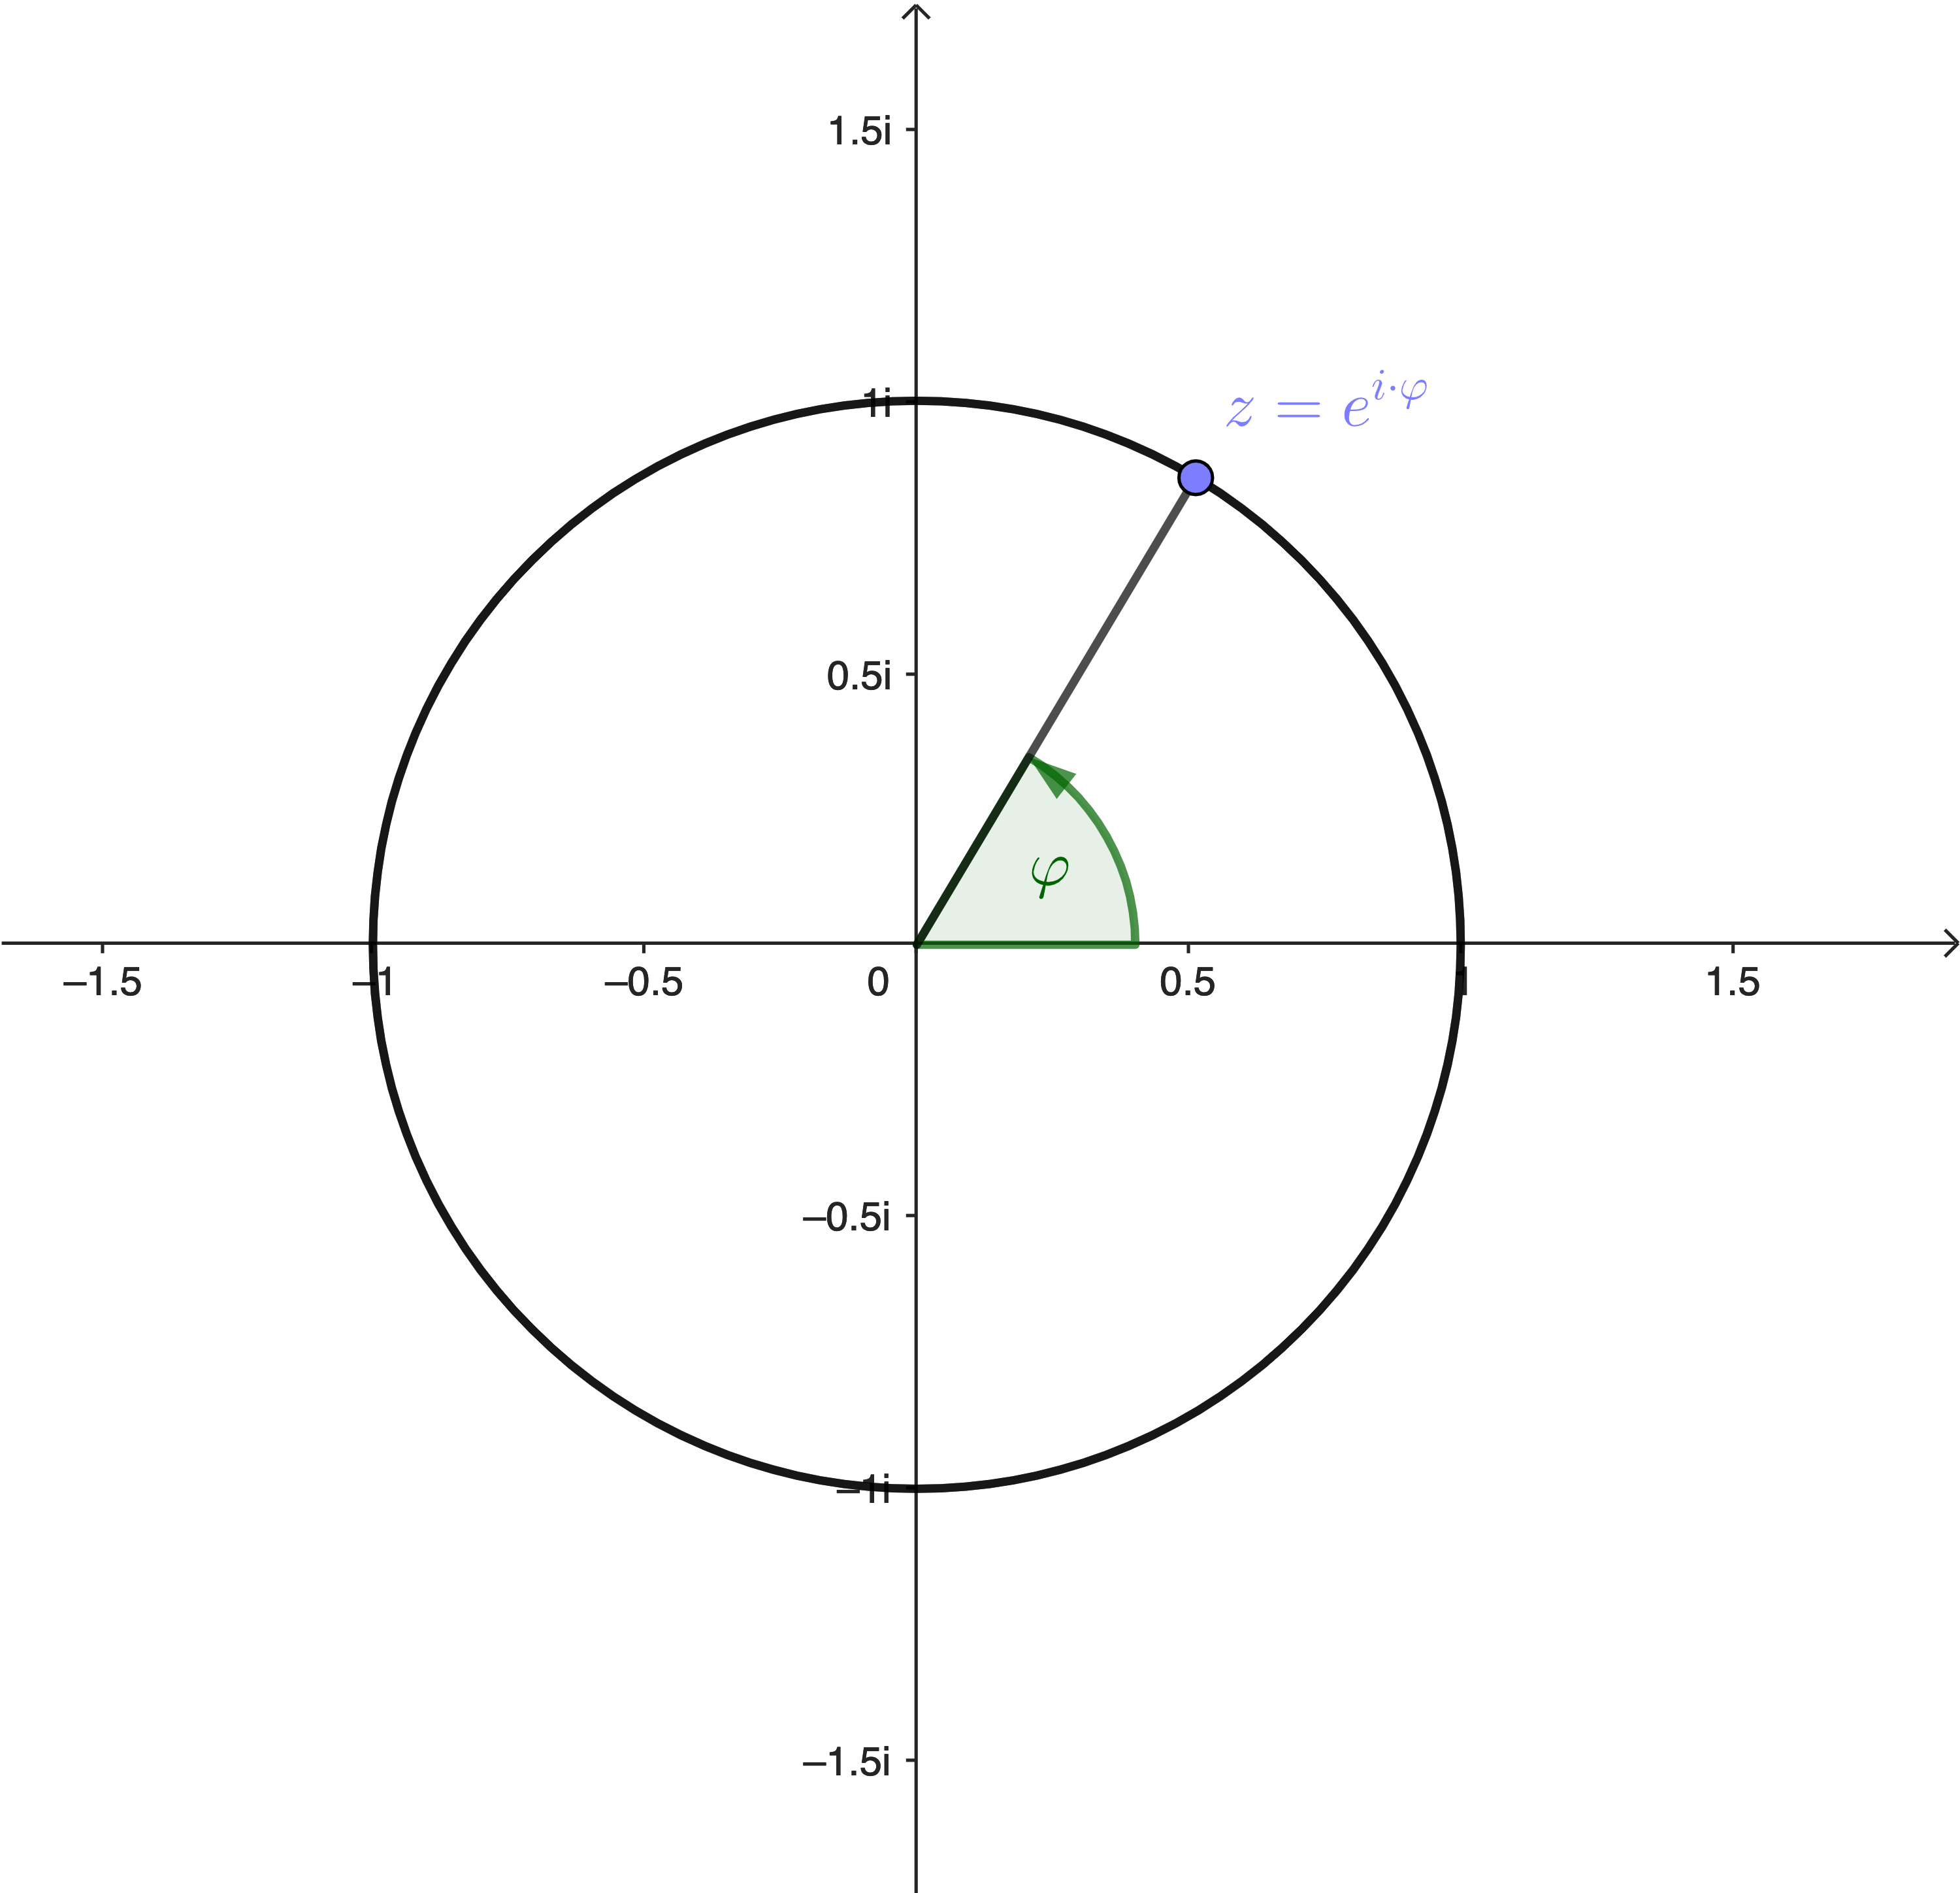
\includegraphics[width = 0.5 \textwidth]{media/eulerformel.png}
	% \end{center}


	\begin{center}
		\begin{tikzpicture}[scale = 1.5]
			% Gitter
			\draw[dashed, very thin, gray] (-2,-2) grid (2,2);

			% Achsen mit Skala
			\draw[->] (-2,0) -- (2,0) node[above] {$\RE$};
			\draw[->] (0,-2) -- (0,2) node[right] {$\IM$};
			\foreach \x in {-1,1}
			\draw (\x,0) -- (\x,-0.2) ;
			\foreach \y in {-1}
			\draw (0,\y) -- (-0.2,\y) ;
			\draw (0,1) -- (-0.2,1) node[above left] {$i$};
			\draw (1,0) -- (1,-0.2) node[below right] {$1$};



			% Einheitskreis
			\draw[dashed] (0,0) circle (1);
			% Punkt z
			\coordinate (z) at (40:1);
			\fill[blue] (z) circle (0.05) node[above right, blue] {$e^{i \cdot \varphi}$};
			\draw[orange](0,0) -- (z);
			\draw[thick, ->, red] (0.5, 0) arc (0:40:0.5) node[midway, right] {$\varphi$};


			%  % Punkt z^2
			%  \coordinate (z2) at (80:1);
			%  \fill[blue] (z2) circle (0.05) node[above right, blue] {$z^2$};
			%  \draw[orange](0,0) -- (z2);
			%  \draw[thick, ->, red] (40:0.5) arc (40:80:0.5) node[midway, above right] {$\varphi$};

			%   % Punkt z^3
			%   \coordinate (z3) at (120:1);
			%   \fill[blue] (z3) circle (0.05) node[above left, blue] {$z^3$};
			%   \draw[orange](0,0) -- (z3);
			%   \draw[thick, ->, red] (80:0.5) arc (80:120:0.5) node[midway, above] {$\varphi$};

		\end{tikzpicture}
	\end{center}
	Im Spezialfall \(\varphi = \pi\)   erhält man die berühmte eulersche Identität:

	\vspace{2 cm}
\end{satz}



\emph{Bemerkungen:}
\begin{itemize}
	\item Die Eulersche Identität vereinigt die „fünf wichtigsten Zahlen des Universums“ in einer einfachen Gleichung. Das Erstaunliche ist, dass diese fünf Zahlen aus ganz verschiedenen Gebieten der Mathematik stammen:
	      \begin{itemize}
		      \item $e$ spielt eine wichtige Rolle in der Differenzialrechnung
		      \item $i$ ist die imaginäre Einheit
		      \item $\pi$ ist die Kreiszahl
		      \item $1$ ist das neutrale Element der Multiplikation
		      \item $0$ ist das neutrale Element der Addition.
	      \end{itemize}
	\item Der Winkel \( \varphi \) ist im Bogenmass.
	\item In Zukunft schreiben wir nicht mehr \( z = r \cdot \text{cis} (\varphi) \), sondern \( z = r\cdot e^{i\varphi} \).
	\item Die Potenzgesetze gelten auch für komplexe Exponenten. Insbesondere gelten die Formeln von De Moivre:
	      \[ e^{i\varphi} \cdot e^{i\psi} = \text{cis}(\varphi) \cdot \text{cis}(\psi) = \text{cis}(\varphi+\psi) = e^{i(\varphi+\psi)} \]
	      \[ (e^{i\varphi})^k = e^{i \cdot k\varphi} \]
\end{itemize}




\clearpage
\begin{ueb}
	{}{}
	\begin{enumerate}
		\item Berechnen Sie den Realteil $\operatorname{Re}(e^{x+iy})$, wobei $x, y \in \mathbb{R}$. Verwenden Sie: $e^{x+iy} = e^x \cdot e^{iy}$.

		\item Berechnen Sie $|e^{i(x+iy)}|$.

		\item Geben Sie eine Lösung der Gleichung $e^z = -2i$ an. Finden Sie auch eine zweite?

		\item Zeigen Sie, dass die Exponentialfunktion $2\pi i$-periodisch ist, das heisst: Für alle $z \in \mathbb{C}$ gilt $e^{z+2\pi i} = e^z$.

		\item Was ist das Bild der folgenden Mengen unter der Exponentialfunktion?
		      \begin{enumerate}
			      \item Imaginäre Achse: $\operatorname{Re}(z) = 0$
			      \item Reelle Achse: $\operatorname{Im}(z) = 0$
			      \item $\operatorname{Re}(z) = 2$
			      \item $\operatorname{Im}(z) = 2$
		      \end{enumerate}
		\item Zur Erinnerung: Die Funktionen Cosinus hyperbolicus und Sinus hyperbolicus sind definiert als:
		      $$ \cosh(x) = \frac{e^x+e^{-x}}{2} \qquad \sinh(x) = \frac{e^x-e^{-x}}{2} $$
		      und es gilt, dass $\cosh'(x) = \sinh(x)$ und $\sinh'(x) = \cosh(x)$.

		      Verwenden Sie die Reihendarstellung von $\sin$ und $\cos$ und die Taylorentwicklung um die Stelle $x_0 = 0$ der Funktionen $\cosh$ und $\sinh$, um zu zeigen, dass für $x\in\R$ gilt:
		      $$\cos(ix) = \cosh(x)\quad\text{und} \quad \frac{\sin(ix)}{i} = \sinh(x)$$

		      %   \begin{enumerate}
		      %       \item Zeigen Sie, dass $\cosh^2(x) - \sinh^2(x) = 1$ ist.
		      %       \item Berechnen Sie die Ableitungen von $\cosh(x)$ und $\sinh(x)$ mit der Kettenregel.

		      %       \item Verwenden Sie die Reihendarstellung von $\sin$ und $\cos$ und die Taylorentwicklung um die Stelle $x_0 = 0$ der Funktionen $\cosh$ und $\sinh$, um zu zeigen, dass für $x\in\R$ gilt:
		      %             $$\cos(ix) = \cosh(x)\quad\text{und} \quad \frac{\sin(ix)}{i} = \sinh(x)$$
		      %   \end{enumerate}
	\end{enumerate}
\end{ueb}

\clearpage
\emph{Lösungen}
\begin{enumerate}
	\item $\operatorname{Re}(e^{x+iy}) = e^x \cos y$
	\item $|e^{i(x+iy)}| = e^{-y}$
	\item $z = \ln(2) + \frac{3\pi}{2} i$. Ausserdem alle Zahlen der Form $z = \ln(2) + \left(\frac{3\pi}{2}+2k\pi\right) i$. Aus diesem Grund gibt es keinen Logarithmus für komplexe Zahlen.
	\item $e^{z+2\pi i} = e^z\cdot e^{2\pi i} = e^z\cdot 1 = e^z$
	\item Bildmengen:
	      \begin{enumerate}
		      \item Einheitskreis
		      \item Positive reelle Achse
		      \item Kreis um den Ursprung mit Radius $e^2$
		      \item Halbgerade $\{t\cdot e ^{2i} | t \in \R^+\}$
	      \end{enumerate}
	\item Die Taylorentwicklung von $\cosh$ lautet:
	      $$\cosh(x) = 1+\frac{x^2}{2!}+\frac{x^4}{4!}+\frac{x^6}{6!} +\dots  $$
	      Wenn man $ix$ in die Reihendarstellung von $\cos$ einsetzt, erhält man:
	      \begin{align*}
		      \cos(ix) & = 1-\frac{(ix)^2}{2!}+\frac{(ix)^4}{4!}-\frac{(ix)^6}{6!} +\dots \\
		               & = 1+\frac{x^2}{2!}+\frac{x^4}{4!}+\frac{x^6}{6!} +\dots          \\
		               & = \cosh(x)
	      \end{align*}
	      Analog für $\sinh$

	      % Cosh und Sinh:
	      %       \begin{enumerate}

	      % 	      \item \begin{align*}
	      % 		            \cosh^2(x) - \sinh^2(x) & =\left(\frac{e^x+e^{-x}}{2}\right)^2 - \left(\frac{e^x-e^{-x}}{2}\right)^2 \\
	      % 		                                    & = \frac{e^{2x} +2 + e^{-2x}}{4} - \frac{e^{2x} - 2 + e^{-2x}}{4}           \\
	      % 		                                    & = \frac{4}{4}                                                              \\
	      % 		                                    & = 1
	      % 	            \end{align*}
	      % 	      \item $(\cosh(x))' = \sinh(x), \quad (\sinh(x))' = \cosh(x)$
	      % 	      \item Die Taylorentwicklung von $\cosh$ lautet:
	      % 	            $$\cosh(x) = 1+\frac{x^2}{2!}+\frac{x^4}{4!}+\frac{x^6}{6!} +\dots  $$
	      % 	            Wenn man $ix$ in die Reihendarstellung von $\sin$ einsetzt, erhält man:
	      % 	            \begin{align*}
	      % 		            \cos(ix) & = 1-\frac{(ix)^2}{2!}+\frac{(ix)^4}{4!}-\frac{(ix)^6}{6!} +\dots \\
	      % 		                     & = 1+\frac{x^2}{2!}+\frac{x^4}{4!}+\frac{x^6}{6!} +\dots          \\
	      % 		                     & = \cosh(x)
	      % 	            \end{align*}
	      % 	            Analog für $\sinh$
	      %   \end{enumerate}
\end{enumerate}




\clearpage
\subsection*{Additum: Matrixexponential}
Die Erweiterung der Exponentialfunktion auf komplexe Argumente (letztes Kapitel) wird die Behandlung von Differentialgleichungen vereinfachen. Bei Systemen von mehreren Differentialgleichungen wird es nützlich sein, Matrizen als Inputs der Exponentialfunktion in Betracht zu ziehen.
\begin{definition}
	{Matrixexponential}{}
	Für eine quadratische Matrix $A$ sei
	$$e^A = \sum_{k=0}^\infty \frac{A^k}{k!} = E + \frac{A}{1!} + \frac{A^2}{2!} + \dots $$
	Wobei $E$ die Einheitsmatrix ist.
\end{definition}
\begin{bsp}
	{Matrixexponential einer nilpotenten Matrix}{}
	Betrachten Sie die Matrix $N$:

	$$
		N = \begin{pmatrix}
			0 & 1 & 0 \\
			0 & 0 & 1 \\
			0 & 0 & 0 \\
		\end{pmatrix}
	$$

	Es gilt
	$$
		N^2 = \begin{pmatrix}
			0 & 0 & 1 \\
			0 & 0 & 0 \\
			0 & 0 & 0 \\
		\end{pmatrix},
		\qquad
		N^3 = \begin{pmatrix}
			0 & 0 & 0 \\
			0 & 0 & 0 \\
			0 & 0 & 0 \\
		\end{pmatrix}
	$$

	Für alle weiteren Potenzen der Matrix gilt dann $N^k=0, \, k\ge3$. Solche Matrizen nennt man \emph{nilpotent}. Die Matrixexponentialfunktion für diese Matrix kann dann wie folgt geschrieben werden:

	$$
		e^N = E + \frac{N}{1!} + \frac{N^2}{2!} = \begin{pmatrix}
			1 & 1 & \frac{1}{2} \\
			0 & 1 & 1           \\
			0 & 0 & 1           \\
		\end{pmatrix}
	$$


\end{bsp}

\begin{bsp}
	{Matrixexponential einer Diagonalmatrix}{eHochDiagonalmatrix}
	Betrachten Sie die Diagonalmatrix $D$:

	$$
		D = \begin{pmatrix}
			1 & 0 \\
			0 & 2 \\
		\end{pmatrix}
	$$

	Dann gilt
	$$ D^k = \begin{pmatrix}
			1 & 0   \\
			0 & 2^k \\
		\end{pmatrix}
	$$

	Das Matrixexponential $e^D$ für diese Matrix kann direkt berechnet werden:

	$$
		e^D = \sum_{k=0}^{\infty} \frac{D^k}{k!} = \begin{pmatrix}
			1 & 0 \\
			0 & 1 \\
		\end{pmatrix} + \frac{\begin{pmatrix}
				1 & 0 \\
				0 & 2 \\
			\end{pmatrix}}{1!} + \frac{\begin{pmatrix}
				1 & 0   \\
				0 & 2^2 \\
			\end{pmatrix}}{2!} + \frac{\begin{pmatrix}
				1 & 0   \\
				0 & 2^3 \\
			\end{pmatrix}}{3!} + \ldots
	$$

	Die Einträge der Matrix $e^D$ lauten dann:
	$$
		e^D = \begin{pmatrix}
			\sum_{k=0}^{\infty} \frac{1}{k!} & 0                                  \\
			0                                & \sum_{k=0}^{\infty} \frac{2^k}{k!}
		\end{pmatrix}
		= \begin{pmatrix}
			e^1 & 0   \\
			0   & e^2 \\
		\end{pmatrix}
	$$
	Wobei im letzten Schritt die Taylorreihe $e^x = \sum_{k=0}^{\infty} \frac{x^k}{k!}$ für $x=1$ und $x=2$ verwendet wurde.
\end{bsp}

\begin{bsp}{Matrixexponential einer diagonalisierbaren Matrix}{}
	Betrachten Sie die  Matrix $A$:

	$$
		A = \begin{pmatrix}
			2 & -1 \\
			0 & 3  \\
		\end{pmatrix}
	$$

	Um die Matrix $e^A$ zu bestimmen, müssen wir $A$ zuerst diagonalisieren. Wie man leicht nachrechnet, hat $A$ die Eigenwerte $\lambda_1 = 2$ und $\lambda_2 = 3$ mit den dazugehörigen Eigenvektoren $\vec{v}_1 = \begin{pmatrix}
			1 \\ 0
		\end{pmatrix}$ und $\vec{v}_2 = \begin{pmatrix}
			-1 \\ 1
		\end{pmatrix}$. Damit gilt
	$$
		A = TDT^{-1} = \begin{pmatrix}
			1 & -1 \\
			0 & 1  \\
		\end{pmatrix} \cdot
		\begin{pmatrix}
			2 & 0 \\
			0 & 3 \\
		\end{pmatrix} \cdot
		\begin{pmatrix}
			1 & -1 \\
			0 & 1  \\
		\end{pmatrix}^{-1}
	$$

	Für $A^2$ gilt dann $A^2 = TD\underbrace{T^{-1} T}_{E} DT^{-1} = TD^2T^{-1}$. Oder allgemein:
	%Damit lassen sich die Potenzen von $A$ leicht berechnen:
	$$
		A^k =TD^kT^{-1}=
		\begin{pmatrix}
			1 & -1 \\
			0 & 1  \\
		\end{pmatrix} \cdot
		\begin{pmatrix}
			2 & 0 \\
			0 & 3 \\
		\end{pmatrix}^k \cdot
		\begin{pmatrix}
			1 & -1 \\
			0 & 1  \\
		\end{pmatrix}^{-1}
	$$

	Für das Matrixexponential gilt nun:

	\begin{align*}
		e^A & = E + \frac{A}{1!} + \frac{A^2}{2!} + \dots                      \\
		    & = TET^{-1} + \frac{TDT^{-1}}{1!} + \frac{TD^2T^{-1}}{2!} + \dots \\
		    & = T\left(E + \frac{D}{1!} + \frac{D^2}{2!} + \dots\right) T^{-1} \\
		    & = T e^D T^{-1}
	\end{align*}
	Das Matrixexponential $e^D$ lässt sich nun leicht wie im Beispiel \ref*{bsp:eHochDiagonalmatrix} berechnen und man erhält schliesslich
	$$
		e^A = T e^D T^{-1} = \begin{pmatrix}
			1 & -1 \\
			0 & 1  \\
		\end{pmatrix} \cdot
		\begin{pmatrix}
			e^2 & 0   \\
			0   & e^3 \\
		\end{pmatrix}\cdot
		\begin{pmatrix}
			1 & -1 \\
			0 & 1  \\
		\end{pmatrix}^{-1} = \begin{pmatrix}
			e^2 & e^2-e^3 \\
			0   & e^3
		\end{pmatrix}
	$$

\end{bsp}
\clearpage
\begin{ueb}
	{}{}
	\begin{enumerate}
		\item Gegeben sei die  $2 \times 2$-Matrix $N$:
		      \[
			      N = \begin{pmatrix} 0 & 0 \\ 4 & 0 \end{pmatrix}
		      \]

		      Berechnen Sie $e^N$.
		\item Gegeben sei die  $3 \times 3$-Matrix $D$:
		      \[
			      D = \begin{pmatrix} 3 & 0 & 0 \\ 0 & -1 & 0 \\ 0& 0 & 0 \end{pmatrix}
		      \]

		      Berechnen Sie $e^D$.
		\item Gegeben sei die  $2 \times 2$-Matrix $A$:
		      \[
			      A = \begin{pmatrix}
				      5  & -2 \\
				      12 & -5
			      \end{pmatrix}
		      \]
		      Berechnen Sie $e^A$.
		\item \emph{Challenge}: Sei $x\in\R$ und $$M = \begin{pmatrix}
				      0 & x \\-x & 0
			      \end{pmatrix}$$
		      Berechnen Sie $e^M$.

		      Tipp: Berechnen Sie einige Matrixpotenten $M^k$ für $k = 1, 2, 3, 4, 5, \dots$ und versuchen Sie, darin ein Muster zu finden.



	\end{enumerate}
\end{ueb}
\clearpage
\emph{Lösungen}
\begin{enumerate}
	\item Da $N^2 = 0$, folgt:

	      \[
		      e^N = E + N + \frac{N^2}{2!} + \frac{N^3}{3!} + \ldots = E + N
	      \]

	      Setzen wir die Werte ein:

	      \[
		      e^N = \begin{pmatrix} 1 & 0 \\ 0 & 1 \end{pmatrix} + \begin{pmatrix} 0 & 0 \\ 4 & 0 \end{pmatrix} = \begin{pmatrix} 1 & 0 \\ 4 & 1 \end{pmatrix}
	      \]

	      Daher ist die Lösung $e^N = \begin{pmatrix} 1 & 0 \\ 4 & 1 \end{pmatrix}$.
	\item $D$ ist eine Diagonalmatrix. Also
	      $$
		      e^D = \begin{pmatrix} e^3 & 0 & 0 \\ 0 & e^{-1} & 0 \\ 0& 0 & e^0 \end{pmatrix} = \begin{pmatrix} e^3 & 0 & 0 \\ 0 & 1/e & 0 \\ 0& 0 & 1 \end{pmatrix}
	      $$
	\item $$ e^A = T e^D T^{-1} = \begin{pmatrix}
			      1 & 1 \\
			      3 & 2 \\
		      \end{pmatrix} \cdot
		      \begin{pmatrix}
			      e^{-1} & 0     \\
			      0      & e^{1} \\
		      \end{pmatrix}\cdot
		      \begin{pmatrix}
			      1 & 1 \\
			      3 & 2 \\
		      \end{pmatrix}^{-1} = \begin{pmatrix}
			      -\frac{2}{e}+3e & \frac{e}{e}-e  \\
			      -\frac{6}{e}+6e & \frac{3}{e}-2e
		      \end{pmatrix}
	      $$
	\item Für die Potenzen $M^0$, $M^1$, $M^{2}$, $M^{3}$, $M^{4}$ und $M^{5}$ erhält man:
	      \begin{align*}
		      M^0 & =  \begin{pmatrix} x^{0} &  0\\ 0 & x^{0} \end{pmatrix}  \\
		      M^1 & = \begin{pmatrix} 0 & x^{1} \\ -x^{1} & 0 \end{pmatrix}  \\
		      M^2 & = \begin{pmatrix}  -x^{2} & 0 \\ 0& -x^{2} \end{pmatrix} \\
		      M^3 & = \begin{pmatrix} 0 & -x^{3} \\ x^{3} & 0 \end{pmatrix}  \\
		      M^4 & = \begin{pmatrix} x^{4} &  0\\ 0 & x^{4} \end{pmatrix}
	      \end{align*}
	      Diese Muster setzt sich so weiter fort. Für jedes $k\in\N$ gilt:
	      \begin{align*}
		      M^{4k}   & = \begin{pmatrix} x^{4k} &  0\\ 0 & x^{4k} \end{pmatrix},       \\
		      M^{4k+1} & = \begin{pmatrix} 0 & x^{4k+1} \\ -x^{4k+1} & 0 \end{pmatrix},  \\
		      M^{4k+2} & = \begin{pmatrix}  -x^{4k+2} & 0 \\ 0& -x^{4k+2} \end{pmatrix}, \\
		      M^{4k+3} & = \begin{pmatrix} 0 & -x^{4k+3} \\ x^{4k+3} & 0 \end{pmatrix}.
	      \end{align*}
	      Damit folgt
	      $$ e^M = \begin{pmatrix}
			      \sum_{k=0}^\infty (-1)^k \frac{x^{2k}}{(2k)!}      & \sum_{k=0}^\infty (-1)^k \frac{x^{2k+1}}{(2k+1)!} \\
			      -\sum_{k=0}^\infty (-1)^k \frac{x^{2k+1}}{(2k+1)!} & \sum_{k=0}^\infty (-1)^k \frac{x^{2k}}{(2k)!}     \\
		      \end{pmatrix}
		      = \begin{pmatrix}
			      \cos(x)  & \sin(x) \\
			      -\sin(x) & \cos(x)
		      \end{pmatrix}
	      $$
\end{enumerate}